\documentclass[
% -- opções da classe memoir --
12pt,				% tamanho da fonte
%openright,			% capítulos começam em pág ímpar (insere página vazia caso preciso)
%openany,
twoside,			% para impressão em verso e anverso. Oposto a oneside
a4paper,			% tamanho do papel.
% -- opções da classe abntex2 --
%chapter=TITLE,		% títulos de capítulos convertidos em letras maiúsculas
%section=TITLE,		% títulos de seções convertidos em letras maiúsculas
%subsection=TITLE,	% títulos de subseções convertidos em letras maiúsculas
%subsubsection=TITLE,% títulos de subsubseções convertidos em letras maiúsculas
% -- opções do pacote babel --
portugues,			% idioma adicional para hifenização
brazil,				% o último idioma é o principal do documento
]{abntex2}

\usepackage[alf]{abntex2cite}	% Citações padrão ABNT

\usepackage{cmap}				% Mapear caracteres especiais no PDF
\usepackage{lmodern}			% Usa a fonte Latin Modern

\usepackage{amsthm}
\usepackage{amsmath}
\usepackage{amsfonts}
\usepackage{amssymb}
\usepackage{algpseudocode}
\usepackage{color}				% Controle das cores
\usepackage{microtype}    % melhorias no micro-espaçamento de texto
%\usepackage{algorithm}
\usepackage[portuguese, ruled, vlined, linesnumbered]{algorithm2e}

\SetKwInput{Kw}{input}

\usepackage{graphicx}			% Inclusão de gráficos
\usepackage{subcaption}

\usepackage[T1]{fontenc}		% Selecao de codigos de fonte.
\usepackage[utf8]{inputenc}		% Codificacao do documento (conversão automática dos acentos)

\definecolor{mylinkcolor}{rgb}{0.05, 0.20, 0.41}
%\definecolor{mylinkcolor}{rgb}{0.04, 0.26, 0.51}
\hypersetup{
    colorlinks=true,
    linkcolor=mylinkcolor,
    filecolor=mylinkcolor,
    urlcolor=mylinkcolor,
    citecolor=mylinkcolor
}


\newtheorem{mydef}{Definição}
\newtheorem{myprop}{Proposição}
\newtheorem{myteo}{Teorema}

\titulo{A Hybrid Heuristic for the Multi-objective Knapsack Problem}
\autor{Marcos Daniel V. Baroni}
\local{Vitória - Espírito Santo - Brasil}
\data{29 de junho de 2018}
\orientador{Dr. Flávio Miguel Varejão}
\instituicao{%
  Universidade Feredal do Espírito Santo -- UFES
  \par
  Departamento de Informática
  \par
  Programa de Pós-Graduação em Informática}
\tipotrabalho{Tese (Doutorado)}
\preambulo{Tese de Doutorado apresentada de acordo
com o regimento do Programa de Pós-graduação
em Informática da Universidade
Federal do Espírito Santo, como requisito para obtenção
do grau de Doutor em Ciência da Computação.}

\makeindex


%%%%%%%%%%%%%%%%%%%%%%%%
% 1. Introdução:
%  (???) Motivação EDP
% 2. MOKP
%   2a. Algoritmos Exatos
%     - Bibliografia
%     - Bazgan's algoritmo
%   2b. Algoritmos Heurísticos
% 3. KDTree
%   3a. Use no Exato
%   3b. Uso no Heurístico
% 4. Experimentos
%   4a. KDT no Exato
%   4b. KDT no Heurístico
% 5. Conclusão
% A. Anexos: Experimentos EDP
%%%%%%%%%%%%%%%%%%%%%%%%

\begin{document}

%%%%%%%%%%%%%%%%%%%%%%%%
% Folhas               %
%%%%%%%%%%%%%%%%%%%%%%%%
\imprimircapa
\imprimirfolhaderosto*

\newcommand{\dtree}[1]{$#1$-d~tree}
\newcommand{\kdtree}{\dtree{k}}
\newcommand{\bsym}[1]{\boldsymbol{#1}}
%\newcommand{\sol}[1]{\boldsymbol{#1}}
\newcommand{\sol}[1]{#1}
\newcommand{\pnt}[1]{pnt(\sol{#1})}
\newcommand{\fsol}[1]{f(\sol{#1})}
\newcommand{\np}{m}
\newcommand{\nphard}{$\mathcal{NP}$-Hard}
\newcommand{\missingI}[1]{}
\newcommand{\missing}[1]{
  \begin{framed}
    {\scriptsize  #1}
  \end{framed}
}
\newcommand{\weight}[1]{w(\sol{#1})}
\newcommand{\obj}[2]{f_{#1}(\sol{#2})}
\newcommand{\bigweight}[1]{w\big(\sol{#1}\big)}
\newcommand{\dom}[2]{dom(\sol{#1}, \sol{#2})}
\newcommand{\domk}[2]{dom_k(\sol{#1}, \sol{#2})}
\newcommand{\setIN}{\{1, \ldots, n\}}
\newcommand{\ext}[2]{ext(\sol{#1}, \sol{#2})}
\newcommand{\domLess}[2]{ \sol{#1} \prec \sol{#2} }
%\newcommand{\logicAnd}{ \textrm{ and } }
\newcommand{\logicAnd}{ \land }
\newcommand{\logicOr}{ \lor}
\newcommand{\solSetA}{ Q }
\newcommand{\solSetB}{ R }
\newcommand{\solSett}{ S_* }
\newcommand{\solSet}{ S }
\newcommand{\rord}{\mathcal{O}_{rev}}
\newcommand{\cb}[2]{cb^{#1}(#2)}  % cost-benefit function
\renewcommand{\leq}{\leqslant}
\renewcommand{\geq}{\geqslant}
\newcommand{\floor}[1]{\left \lfloor{#1}\right \rfloor}

% bar graphs configs
\newcommand{\cmpH}{4.0cm}
\newcommand{\cmpW}{7cm}
\newcommand{\legX}{0.45}
\newcommand{\legY}{-0.30}
\newcommand{\scecore}{SCEcr }
\newcommand{\mokp}{MOKP}
\newcommand{\paretoset}{conjunto Pareto}
\newcommand{\paretosetII}{conjunto Pareto-ótimo}
\newcommand{\knapsackdominates}{domina segundo a mochila}

% big bullet
\newcommand{\bbt}{\,\begin{picture}(-1,1)(-1,-2)\circle*{5}\end{picture}\ }

\newpage \phantom{a}
\begin{folhadeaprovacao}

  \begin{center}
    {\ABNTEXchapterfont\large\imprimirautor}

    \vspace*{\fill}\vspace*{\fill}
    {\ABNTEXchapterfont\bfseries\Large\imprimirtitulo}
    \vspace*{\fill}
    
    \hspace{.45\textwidth}
    \begin{minipage}{.5\textwidth}
        \imprimirpreambulo
    \end{minipage}%
    \vspace*{\fill}
   \end{center}
    
   Work approved. \imprimirlocal, November 27, 2017:

   \assinatura{\textbf{\imprimirorientador} \\ Advisor} 
   \assinatura{\textbf{Dr.ª Simone de Lima Martins} \\ Guest}
   \assinatura{\textbf{Dr. Arlindo Gomes de Alvarenga} \\ Guest}
   %\assinatura{\textbf{Professor} \\ Convidado 3}
   %\assinatura{\textbf{Professor} \\ Convidado 4}
      
   \begin{center}
    \vspace*{0.5cm}
    {\large\imprimirlocal}
    \par
    {\large\imprimirdata}
    \vspace*{1cm}
  \end{center}
  
\end{folhadeaprovacao}


\begin{resumo}
Diversos problemas reais envolvem a otimização simultânea de múltiplos critérios,
os quais são, geralmente, conflitantes entre si.
Estes problemas são denominados multiobjetivo e
não possuem uma única solução, mas um conjunto de soluções de interesse, denominadas soluções
eficientes ou não dominadas.
Um dos grande desafios a serem enfrentados na resolução deste tipo de problema é o
tamanho do conjunto solução, que tende a crescer rapidamente dado o tamanho da instância,
degradando a performance dos algoritmos.
Dentre os problemas multiobjetivos mais estudados está o problema da mochila multiobjetivo,
pelo qual diversos problemas reais podem ser modelados.
Este trabalho propõe a aceleração do processo de solução do problema da mochila multiobjetivo,
através da utilizando da \kdtree{} como estrutura de indexação multidimensional
para auxiliar a manipulação das soluções.
A performance da abordagem é analisada através de experimentos
computacionais, realizados no contexto exato utilizando um algoritmo estado da arte.
Testes também são realizados no contexto heurístico, utilizando a adaptação
de uma meta-heurística para o problema em questão, sendo esta também uma contribuição do presente trabalho.
Segundo os resultados, para o contexto exato a proposta foi eficaz, apresentam speedup de até $2.3$
para casos bi-objetivo e $15.5$ em casos 3-objetivo, não sendo porém
eficaz no contexto heurístico, apresentando pouco impacto no tempo computacional.
Em todos os casos, porém, houve considerável redução no número de avaliações de soluções.

\vspace{\onelineskip}

\noindent
\textbf{Palavras Chave}:
Problema da Mochila Multiobjetivo,
Indexação Multidimensional,
Meta-heurística,
Algoritmo Exato.
\end{resumo}


\begin{resumo}[Abstract]
\begin{otherlanguage*}{english}
Several real problems involve the simultaneous optimization of multiple criteria,
which are generally conflicting with each other.
These problems are called multiobjective and
do not have a single solution, but a set of solutions of interest, called efficient solutions
or non-dominated solutions.
One of the great challenges to be faced in solving this type of problem is the
size of the solution set, which tends to grow rapidly given the size of the instance,
degrading algorithms performance.
Among the most studied multiobjective problems is the multiobjective knapsack problem,
by which several real problems can be modeled.
This work proposes the acceleration of the resolution process of the multiobjective knapsack problem,
through the use of a \kdtree {} as a multidimensional index structure
to assist the manipulation of solutions.
The performance of the approach is analyzed through computational experiments,
performed in the exact context using a state-of-the-art algorithm.
Tests are also performed in the heuristic context, using the adaptation
of a meta-heuristic for the problem in question, being also a contribution of the present work.
According to the results, the proposal was effective for the exact context, presenting a speedup up to $2.3$
for bi-objective cases and $15.5$ for 3-objective cases, but not
effective in the heuristic context, presenting little impact on computational time.
In all cases, however, there was a considerable reduction in the number of solutions evaluations.
\vspace{\onelineskip}

\noindent

\textbf{Keywords}:
Multiobjective Knapsack Problem,
Multidimensional Indexing,
Metaheuristic,
Exact Algorithm.
\end{otherlanguage*}
\end{resumo}

% Falar brevemente sobre o MOKP
% Falar brevemente sore a estratégia de indexação
% Resumir os resultados obtidos

%\missingt{
%Observar as 5 regras:\\
%1. A general statement introducing the broad research area of the particular topic being investigated;\\
%2. An explanation of the specific problem (difficulty, obstacle, challenge) to be solved;\\
%3. A review of existing or standard solutions to this problem and their limitations;\\
%4. An outline of the proposed new solution;\\
%5. A summary of how the solution was evaluated and what the outcomes of the evaluation were.
%}

% 1. Uma declaração geral introduzindo a área de pesquisa;
% 2. Uma explicação espeficica do problema
% 3.
%
%

%%%%%%%%%%%%%%%%%%%%%%%%
%  Sumário             %
%%%%%%%%%%%%%%%%%%%%%%%%
\pdfbookmark[0]{\contentsname}{toc}
\tableofcontents*

%%%%%%%%%%%%%%%%%%%%%%%%
%  Texto               %
%%%%%%%%%%%%%%%%%%%%%%%%
% Introdução
\chapter{Introdução}
%  - The problem and its application
%  - Literature background
%  - The Bazgan algorithm
%  - Our approach (motivation and use of KDTRee)
%  - Article structure


% Multi-objective Knapsack Problem
\chapter{Problema da Mochila Multi-objetivo}
% Breve definicao de multiobjective opt
A general multiobjective optimization problem can be described as a vector
function $f$ that maps a tuple of $n$ parameters (decision variables) to a tuple
of $\np$ objectives.
Formally:
\begin{align*}
  \text{min/max} ~ \sol{y} &= f(\sol{x}) = 
    \big(f_1(\sol{x})
    ,f_2(\sol{x})
    ,\ldots
    ,f_{\np}(\sol{x})\big) \\
  \text{subject to} ~ \sol{x} & = (x_1, x_2, \ldots, x_n) \in X
\end{align*}
where $\sol{x}$ is called the \emph{decision vector} or \emph{solution}, $X$ denotes the set
of feasible solutions, and $\sol{y}$ is the \emph{objective vector} or \emph{criterion vector} where
each objective has to be minimized (or maximized).

Considering two decision vectors $\sol{a}, \sol{b} \in X$, $a$ is said to
\emph{dominate} $b$ if, and only if:
\begin{align*}
    \forall i &\in \{1, 2, \ldots, \np\}: f_i(\sol{a}) \geq f_i(\sol{b}) \\
    \exists j &\in \{1, 2, \ldots, \np\}: f_j(\sol{a}) > f_j(\sol{b})
\end{align*}

A solution $\sol{a} \in X$ is called \emph{efficient} or \emph{non-dominated}
if there is not other feasible solution $\sol{b} \in X$ such that $\sol{b}$ dominates $\sol{a}$.
The set of solutions of a multiobjective optimization problem consists of all efficient solutions.
This set is known as \emph{Pareto optimal}.

The instance of a multiobjective knapsack problem with $\np$
objectives consists of an integer capacity $W > 0$ and $n$ items.
Each item $i$ has a positive weight $w^i$ and $\np$ non negative integer
profits $p_{i}^{1}, \ldots, p_{i}^{\np}$.
A solution is represented by a vector $\sol{x} = (x_1, \ldots, x_n)$ of binary
decision variables $x_i$, such that $x_i = 1$ if item $i$ is included in the
solution and $0$ otherwise, satisfing the capacity of the knapsack.
For any instance of the problem, we aim at determining the set of efficient solutions.

Formally the definition of the problem is:
\begin{align*}
    \text{max   } & f(\sol{x}) = 
      \big(f_1(\sol{x}) ,f_2(\sol{x}) ,\ldots ,f_{\np}(\sol{x})\big) \\
    \text{subject to   } & w(\sol{x}) < W \\
    & x_{i} \in \{0, 1\} \quad i = 1, \ldots, n \\
    \text{where} \phantom{mmmmm} \\
    f_j(\sol{x}) &= \sum_{i=1}^{n} v^j_i x_i \quad j = 1, \ldots, \np \\
    w(\sol{x}) &= \sum_{i=1}^{n} w_i x_i
\end{align*}

The MOKP is considered a \nphard{} problem, since it is a generalization
of the well-known 0$-$1 knapsack problem and
it is quite difficult to determine the Pareto optimal set for the MOKP,
especially for high dimension instances, in which the Pareto set it self tends
to grow exponentially.
For this reason, the development of methods efficiently deal with high-dimension
instances is...

% Definições, Propriedados e teoremas para o MOKP: dominancia


\section{Métodos Exatos}
\missing{Comentar sobre background de propostas de métodos exatos.}

\missing{Comentar sobre o método da Bazgan como sendo considerado o melhor, citar melhorias propostas.}

O algoritmo de Nemhauser e Ullmann é um algorimto de programação dinâmica
que resolve problemas da mochila de forma genérica aplicando o conceito de
dominância da mochila para remover soluções parciais que não resultarão em
soluções eficientes, ou seja, soluções que irão compor o \paretoset{} (conjunto solução).

\begin{algorithm}
  \caption{O algoritmo de Nemhauser e Ullmann para o \mokp.}
  \label{alg:nemull}
  \Kw{$\bsym{p}, \bsym{w}, W$}
\Begin{
  \SetAlgoLined
  $S_0 = \{(0, \ldots, 0)\}$\;
  \For{$k \gets 1, n$}{
    $S_k \gets S_{k-1} \cup \big\{(s^1 + p_k^1, \ldots, s^\np + p_k^\np, s^{\np+1} + w_k)\;$\
    $\phantom{S_k \gets S_{k-1} \cup \;} \big| \; s^{\np+1} + w_k \leq W, \: s \in S_{k-1} \big\}$\;
  }
  $P = \{ s \in S_n \:|\: \nexists (a \in S_n \;|\; a \dom s)\}$\;
  \textbf{return} $P$\;
}

\end{algorithm}

O algoritmo inicia definindo uma solução inicial $S^0$ contendo apenas a solução
vazia (linha 2).
Na $k$-ésimo iteração o algoritmo recebe um conjunto $S^{k-1}$ contendo
soluções exclusivamente compostas pelos primeiros ${k-1}$ itens,
ou seja, $\forall\sol{x} \in S^{k-1}, \sol{x} \subseteq \{1, \ldots, k-1\}$.
O conjunto $S^{k-1}$ é então expandido adicionando-se uma cópia de cada uma
das suas soluções mas desta vez incluindo o $k$-ésimo item (linha 4),
formando o conjunto $S^k_*$, o qual possui o dobro da cardinalidade de $S^{k-1}$.
O conjunto $S^k_*$ é então reduzido, retirado-se todas as soluções que são dominadas
(segundo a dominância da mochila) por alguma outra (linha 5).
Após a conclusão das iterações um passo final remove as soluções inviáveis
e também as dominadas por alguma outra, dessa vez porém, considerando apenas os
valores de lucro (linha 7).

Apesar de sua simplicidade o Algoritmo~\ref{alg:nemull} é consideravelmente poderoso.
Contudo o potencial crescimento exponencial do \paretoset{} para o \mokp
compromete severamente o seu desempenho.
Uma forma de atacar este problema é tentar reduzir ainda mais a quantidade de
soluções parciais manuseadas durante as iterações do algoritmo.
\missing{ Falar sobre as 3 propostas de redução de número de soluções da bazgan
e justificar as definições seguintes. }


\missing{Explicar que o algoritmo Bazgan considera um conceito generalizado
de dominância aplicado a cada iteração.}

O processo sequencial executado pelo algoritmo de programação dinâmica
consiste de $n$ iterações.
A cada $k$-ésima iteração é gerado o conjunto de estados $S^k$,
que representa todas as soluções viáveis compostas de itens exclusivamente
pertencentes aos $k$ primeiros itens ($k = 1, \ldots, n$).
Um estado $s_k = (s_k^1, \ldots, s_\np^k, s_{\np-1}^k) \in S_k$ represena uma solução
viável que tem valor $s^i_k$ como $i$-ésimo objetivo ($i = 1, \ldots, \np$)
e $s^{\np-1}_k$ de peso.
Portanto, temos $S_k = S_{k-1} \cup \{(s^1_{k-1}+p^1_k)\}$

\missing{Comentar sobre as estratégias de redução dos conjuntos
de estados, motivando as definições a seguir.}

\begin{mydef}[Extensão, Restrição e Complemento]
Considere o Algoritmo~\ref{alg:nemull} e qualquer estado $s_k \in S_K (k < n)$.
Um \emph{complemento} de $s_k$ é qualquer subconjunto  $J \subseteq \{k+1, \ldots, n\}$
tal que $s_k^{\np+1} + \sum_{j \in J} w_j \leq W$.
Assumiremos que qualquer estado $s_n \in S_n$ admite o conjunto vazio como único complemento.
Um estado $s_n \in S_n$ é uma \emph{extensão} de $s_k \in s_k (k \leq n )$ se, e somente se,
existe um complemento $J$ de $s_k$ tal que $s_n^i = s_k^i + \sum_{j \in J} p_j^i) para \; i = 1, \ldots, \np$
e $s_n^{p+1} = s_k^{p+1} + \sum_{j \in J} w_j$.
O conjunto de extenções de $s_k$ é denotado por $Ext(s_k) (k \leq n)$.
Um estado $s_k \in S_k (k \leq n)$ é uma \emph{restrição} do estado $s_n \in S_n$
se, e somente se, $s_n$ é uma extenão de $s_k$.
\end{mydef}

\begin{mydef}[Relação de dominância entre soluções]
\end{mydef}

\subsection{}

\section{Métodos Heurísticos}
Uma das principais dificuldades encontradas no problema da mochila multiobjetivo
é a grande cardinalidade do \paretoset{}.
De fato, grande parte dos problemas multiobjetivos são considerados \emph{intratáveis},
no sentido de possuir uma quantidade exponencial de soluções eficientes
dado o tamanho da instância~\cite{ehrgott2013multicriteria}.
Esta causa tem motivado pesquisadores
a desenvolverem métodos heurísticos, que computam aproximações deste conjunto
demandando menor esforço computacional quando comparado aos métodos exatos.
%~\cite{bazgan2015approximate, vanderpooten2017covers}.

A maioria das heurísticas propostas para problemas multiobjetivo
são adaptações de meta-heurísticas originalmente propostas para
problemas de otimização escalar.
Dentre esses métodos vale mencionar o algoritmo de recozimento simulado
~\cite{czyzzak1998pareto},
o algoritmo de busca dispersa~\cite{da2006scatter,da2007integrating},
algoritmo de busca tabu~\cite{gandibleux2000tabu},
algoritmo imunológico artificial~\cite{gao2014quantum},
algoritmo genético~\cite{abdelaziz1999hybrid}
e o algoritmo de estimação de distribuição~\cite{martins2017hybrid}.

Uma das heurísticas mais populares para o MOKP é o algoritmo genético
de ordenação não dominada (NSGA-II) proposto em~\cite{deb2002fast}.
O NSGA-II se diferencia das primeiras propostas de algoritmos evolucionários
multiobjetivo por utilizar uma estratégia mais eficiente
de ordenação de soluções dominantes e, consequentemente de
definição de aptidão do indivíduo.
O processo de ordenação de soluções dominantes agrupa as soluções
em conjuntos ordenados, chamados \emph{frontes não dominados},
nos quais as soluções dos primeiros conjuntos não são dominadas pelas soluções dos conjuntos seguintes.
A estratégia consiste em realizar um pré-processamento sobre o conjunto de
soluções, no qual são computados para cada solução $x$ dois parâmetros: a quantidade de soluções
que dominam $x$ e o conjunto de soluções dominadas por $x$.
Este pré-processamento permite a otimização do procedimento de ordenação.
Sendo $\np{}$ o número de objetivos e $N$ o tamanho da população,
o procedimento de ordenação proposto requer apenas $\mathcal{O}(\np{}N^2)$ comparações
enquanto que os procedimentos anteriormente utilizados demandavam $\mathcal{O}(\np{}N^3)$ comparações.

Com o objetivo de manter a diversidade das soluções,
o NSGA-II também propõe a utilização de uma métrica de distância entre os indivíduos da população
baseada na média das distâncias entre uma solução e suas
vizinhas imediatas pertencentes ao mesmo fronte não dominado.
A média calculada caracteriza uma espécie de \emph{medida de aglomeração}.
Soluções rodeadas por outras soluções próximas possuem um alto valor de aglomeração,
enquanto soluções que apresentam uma vizinhança distante possuem baixo valor de aglomeração.
O algoritmo então tende a dar preferência às soluções com menor valor de aglomeração,
uma vez que manter soluções com alto valor de aglomeração tende a diminuir a diversidade do conjunto de soluções.
O NSGA-II então implementa um algoritmo genético com abordagem elitista,
%Inicialmente uma população de $N$ indivíduos é criada.
%Em seguida uma nova população de $N$ indivíduos é gerada a partir da população anterior.
%Os indivíduos da nova população juntamente com os da população anterior têm suas aptidões computadas
%através da ordenação em frontes não dominados.
%Os $N$ indivíduos com melhor valor de aptidão são então selecionados,
considerando quando necessário, a métrica proposta como critério de desempate.

Outra heurística popular para o MOKP é o algoritmo evolucionário de pareto robusto
(SPEA-II), proposto em~\cite{zitzler2001spea2}.
O SPEA-II mantém durante o processo de otimização um conjunto de tamanho limitado,
desassociado da população corrente, contendo soluções não dominadas encontradas durante o processo.
Este conjunto, chamado de \emph{arquivo externo}
ou somente \emph{arquivo} (\emph{external archive} ou \emph{archive} em inglês)
é atualizado ao final de cada etapa de evolução, quando os melhores
indivíduos da população corrente são tomados como candidatos para inserção nesse arquivo.

O SPEA-II também propõe utilizar um valor refinado de aptidão.
Para as soluções não-dominadas, o valor de aptidão é associada
ao número de soluções da população que são dominadas pela respectiva solução.
Para os indivíduos dominados, o valor de aptidão é calculado com base nos valores de aptidão
das respectivas soluções dominantes.
Como critério de desempate é utilizada uma métrica de densidade, baseada na distância
até os $k$ vizinhos mais próximos.
Assim que o processo evolutivo se encerra, o SPEA-II retorna o arquivo externo como sendo a aproximação do \paretoset.

Outro algoritmo heurístico popular, para o qual se relata os melhores desempenhos para o MOKP,
é o algoritmo multiobjetivo evolucionário baseado em decomposição (MOEA/D)~\cite{zhang2007moea}.
O MOEA/D decompõe o problema original em $N$ subproblemas escalares, utilizando
um vetor de coeficientes de agregação.
Esses $N$ subproblemas são solucionados
através da evolução simultânea de $N$ populações, uma população para cada subproblema.
A cada geração a população é composta pelo melhor indivíduo encontrado até o momento
para aquele determinado subproblema, o que garante a convergência em direção ao \paretoset{}.
Além disso são definidas relações de vizinhança entre os subproblemas, baseadas
nas distâncias entre seus vetores de agregação.
Durante o processo de evolução, são utilizadas informações de subproblemas vizinhos,
fazendo com que dois subproblemas vizinhos tenham soluções similares.
O trabalho ainda discute diferentes estratégias para se definir os vetores de agregação.

Recentemente foi proposta uma heurística cooperativa para o MOKP baseado
em inteligência de enxame (MOFPA)~\cite{zouache2018cooperative},
apresentando resultados superiores às demais heurísticas.
O MOFPA combina a estratégia de movimento utilizada na otimização
por enxame de partículas com a estratégia de movimento
utilizada pelo algoritmo de otimização por colônia de vaga-lumes.
O algoritmo mantém uma população de indivíduos cujas posições
são atualizadas segundo a influência de outros indivíduos da população,
em uma movimentação par-a-par.
A estratégia de movimento a ser aplicada é definida
segundo a relação de dominância entre os dois indivíduos:
caso o indivíduo a ser movimentado domine o outro, o cálculo de movimento
é feito segundo o método de otimização por enxame de partículas,
caso contrário, o indivíduo é movimentado segundo o cálculo de atratividade
entre indivíduos, definido pelo algoritmo de colônia de vaga-lumes.
Visto que o movimento dos indivíduos ocorre em um espaço
contínuo, uma função de transição é aplicada para discretização da solução.
A estratégia de arquivo externo de soluções não dominadas
é utilizada para garantir as melhores soluções encontradas durante o processo de evolução,
assegurando assim a convergência do método em direção ao \paretoset{}.
Segundo os resultados computacionais apresentados,
o MOFPA foi capaz de gerar soluções
que superam diversas soluções estabelecidas pelos métodos anteriores.

\missingf{Eu acho que passa assim, mas vc está perdendo oportunidade de dar um maior volume na sua tese.
Como vc utiliza esses algoritmos nos experimentos poderia detalhar mais a sua descricao. Apresentar os algoritmos. Nao deve ser tao detalhado qto o do SCE mas pode ser bem mais detalhado do que vc fez. Sua tese está com 55 paginas... Tem que ser algo muito bom (com bons resultados) para passar sem problemas.

\resp Eu não utilizei nenhum dos algoritmos, utilizei apenas os resultados que o Zouache me enviou por email.

F: K, não utilizou, mas se explicar bem como funciona ajuda quem lê a compreender o que esses algoritmos fazem e o que o seu nao faz.

Sim, vou detalhar mais cada um deles. Cerca de três parágrafos para cada algoritmo, está bom?

F: Acho pouco mas melhor que nada. Prefiriria que incluisse os algoritmos na descricao.

}

Uma das propostas do presente trabalho é a implementação de um algoritmo evolutivo
populacional chamado algoritmo de evolução estocástica por complexos,
\emph{shuffled complex evolution} (SCE) em inglês,
para o problema da mochila multiobjetivo.
O SCE é uma heurística evolutiva robusta que surgiu como proposta
de solução para problemas hídricos de modelagem complexa~\cite{duan1992effective} e
deste então tem sido utilizada em outros problemas de otimização escalar.
Na seção seguinte o SCE será apresentado bem como as propostas de adaptação para ser aplicado ao
caso multiobjetivo e de implementação para o MOKP.

Esta proposta de implementação do algoritmo SCE para o MOKP será utilizada para testar o
desempenho da indexação multidimensional para o MOKP no contexto heurístico.
Visando validar a heurística proposta, sua performance com relação à qualidade de solução
também será comparada às principais heurísticas da literatura, cujos resultados serão
apresentados no Capítulo~\ref{cap:exp}.

\subsection{Evolução Estocástica por Complexos}

O Algoritmo de evolução estocástica por complexos (SCE)
é um algoritmo evolutivo populacional originalmente proposto por Duan~\cite{duan1992effective}
para auxiliar o planejamento de modelos de escoamento de águas pluviais.
Esse algoritmo tem sido utilizado com sucesso em diversos problemas como
seleção de projetos~\cite{elbeltagi2007modified},
problemas de escalonamento \cite{zhao2015shuffled},
problema da mochila $0-1$~\cite{bhattacharjee2014shuffled} e
problema da mochila multi-dimensional~\cite{baroni2015shuffled,baroni2016shuffled}.

O SCE é inspirado na evolução natural que ocorre de forma simultânea em
comunidades independentes.
A Figura~\ref{img:flow1} apresenta um fluxograma resumido do SCE.
O algoritmo trabalha com uma população particionada em $N$ comunidades,
ou complexos, cada uma contendo $M$ indivíduos.
Inicialmente a população de $N*M$ indivíduos é tomada aleatoriamente do espaço
de soluções viáveis.
Após essa inicialização, a população é ordenada em ordem decrescente de aptidão
e o melhor global é identificado.
Toda a população é então particionada em $N$ complexos, cada um contendo $M$ indivíduos.
Nesse processo de distribuição ocorre uma operação de \emph{embaralhamento} (\emph{shuffling} em inglês)
dos indivíduos, no qual o primeiro indivíduo é incluído no primeiro complexo,
o segundo indivíduo no segundo complexo, o $M$-ésimo
indivíduo no $M$-ésimo complexo, o $M+1$-ésimo indivíduo no primeiro complexo,
e assim por diante.

O próximo passo após a distribuição dos indivíduos em complexos é evoluir cada
complexo $K'$ vezes, sendo $K'$ uma constante.
Nesse processo, considerando que os indivíduos em cada complexo estão ordenados
em ordem decrescente de aptidão, um subcomplexo de $P$ indivíduos é selecionado
dentre o respectivo complexo, utilizando uma distribuição triangular, em que o $i$-ésimo
indivíduo tem a probabilidade $p_i = \frac{2(n+1-i)}{n(n+1)}$ de ser selecionado.
A utilização da distribuição triangular tem por objetivo priorizar os indivíduos
com melhor aptidão, favorecendo assim a convergência do algoritmo.

Após a seleção do subcomplexo, o seu pior indivíduo é identificado para ser
substituído por um novo indivíduo.
Esse novo indivíduo é gerado através do cruzamento do pior com um outro
de melhor aptidão.
Primeiramente o melhor indivíduo do subcomplexo é considerado.
Caso o indivíduo gerado não seja melhor que o pior selecionado,
o melhor indivíduo do complexo é então usado no cruzamento.
Se esse último cruzamento não resultou em melhoria, o melhor indivíduo de toda
a população é utilizado.
Finalmente, se todos os cruzamentos não foram capazes de gerar um melhor indivíduo,
esta pior solução selecionada é substituída por um novo indivíduo retirado de
forma aleatória do espaço de soluções viáveis.
Esse último procedimento é importante para impedir que o algoritmo fique
\emph{preso} num ótimo local.
O procedimento de evolução descrito acima é apresentado no fluxograma da Figura~\ref{img:flow2}.

\begin{figure}
  \centering
  \begin{minipage}[b]{0.42\textwidth}
    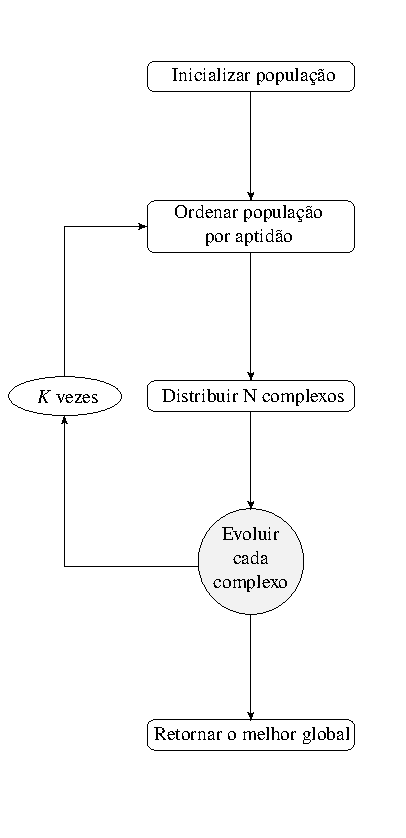
\includegraphics[width=\textwidth]{img/sce/flow1}
    \caption{Algoritmo de evolução estocástica por complexos.}
    \label{img:flow1}
  \end{minipage}
  \hfill
  \begin{minipage}[b]{0.42\textwidth}
    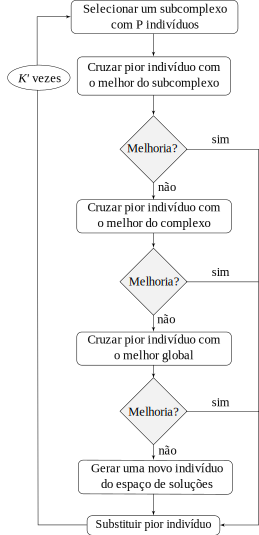
\includegraphics[width=\textwidth]{img/sce/flow2}
    \caption{Etapa de evolução executada para cada um dos complexos.}
    \label{img:flow2}
  \end{minipage}
\end{figure}

Após evoluir todos os $N$ complexos toda a população é novamente ordenada
em ordem decrescente de aptidão e o processo continua até que a condição
de parada seja satisfeita.
Destaca-se que no fluxograma da Figura~\ref{img:flow1} a condição de parada é a
execução de uma quantidade fixa de $K$ evoluções.

Uma das adaptações necessárias para se aplicar o SCE a um problema multiobjetivo
é a redefinição de métrica de qualidade de solução (aptidão),
uma vez que esta não é explícita como no caso da otimização escalar.
A métrica utilizada nesta proposta será a mesma adotada por heurísticas como NSGA-II e MOFPA,
a qual se baseia na ordenação não dominada (\emph{nondominated sorting}, em inglês)
das soluções, por apresentarem os melhores resultados relatados na literatura.

A ordenação não dominada agrupa as soluções em conjunto chamados \emph{frontes não dominados},
os quais possuem uma ordenação de dominância entre si. O primeiro fronte é formado
pelas soluções não dominadas.
Já o segundo fronte é formado pelas soluções dominadas apenas pelo primeiro fronte.
O terceiro fronte, por sua vez, é formado pelas soluções dominadas pelo primeiro
e segundo fronte, e assim sucessivamente.
Dessa forma as soluções dos frontes anteriores são consideradas superiores às soluções
dos frontes posteriores.

O Algoritmo~\ref{alg:frontsort} apresenta o algoritmo proposto por~\cite{deb2002fast}
e utilizado neste trabalho para ordenar as soluções em frontes não dominados.
A primeira fase do algoritmo é apresentada nas linhas 2 a 8,
onde algumas informações são pré-computadas.
Nas linhas 9 a 17 executa-se a segunda fase do algoritmo, onde as soluções são finalmente agrupadas
nos frontes.
Primeiramente são inicializados para cada solução $i$
os contadores de soluções dominadas $n_i$ (linha 2) e
o conjunto de soluções dominantes $B_i$ (linha 3).
Em seguida é feita uma comparação par-a-par através dos laços das linhas 4 e 5
para verificar se uma solução domina a outra (linha 6).
Caso isso aconteça, o contador de soluções dominantes e o conjunto de suas soluções dominadas
é atualizado.
Em seguida é definido o primeiro fronte de pareto, formado pelas soluções
não dominadas por nenhuma outra, ou seja, soluções que tem $n_i = 0$ (linha 9).
Enquanto houver alguma solução com ao menos uma solução dominante registrada (linha 11)
o algoritmo define um novo fronte (linhas 12 a 16).
Para cada solução que compõe o fronte anterior (linha 13), a lista de soluções dominadas
é visitada (linha 14), decrementando-se seus contadores de dominantes (linha 15).
Esse último passo faz com que a contagem de soluções dominantes $n_i$ desconsidere
as soluções recém agrupadas.
Na linha 16 o novo fronte é definido.
Quando todas as soluções estiverem agrupadas em frontes, o algoritmo é encerrado,
retornando a lista de frontes.

\begin{algorithm}
  \Kw{$A = (a_1, \ldots, a_q):$ conjunto de soluções }
\KwResult{$(F_1, \ldots, F_k ):$ Lista de frontes de pareto }
\Begin{
  $n_1, \ldots, n_q \gets 0$;\\
  $B_1, \ldots, B_q \gets \{\}$;\\
  \For{ $i \gets 1 : q$ }{
    \For{ $j \gets 1 : q$ }{
      \If{$a_i \;\dom\; a_j$}{
        $n_j \gets n_j + 1$;\ \mycomment[7.2mm]{ quantidade de soluções que dominam $a_j$ }
        $B_i \gets B_i \cup \{a_j\}$;\ \mycomment[1.2mm]{ conjunto das soluções dominadas por $a_i$ }
      }
    }
  }
  $ k \gets 1$;\\
  $F_1 \gets \{ a_i \in A \;|\; n_i = 0\}$;\ \mycomment[6.5mm]{ soluções não-dominadas (1º fronte) }
  \While{$\exists i \in \{1, \ldots, q\} \;|\; n_i > 0$}{
    $k \gets k + 1$\;
    \For{$a_i \in F_{k-1}$}{
      \For{$ a_j \in B_i$}{
        $n_j \gets n_j - 1$;\ \mycomment[7.2mm]{atualizando contagem}
      }
    }
    $F_k \gets \{ a_i \in A \;|\; n_i = 0\}$;\ \mycomment{formação do kº fronte}
  }
  \textbf{return} $(F_1, \ldots, F_k)$\;
}
  \caption{Algoritmo de ordenação de soluções em frontes não dominados.}
  \label{alg:frontsort}
\end{algorithm}

\begin{figure}
  \centering
  \begin{minipage}[t]{0.48\textwidth}
    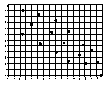
\includegraphics[width=\textwidth]{img/sce/unrankpop}
    \caption{População sem ordenação.}
    \label{img:unrankpop}
  \end{minipage}
  \hfill
  \begin{minipage}[t]{0.48\textwidth}
    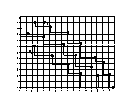
\includegraphics[width=\textwidth]{img/sce/rankpop}
    \caption{População ordenada em frontes não dominados.}
    \label{img:rankpop}
  \end{minipage}
\end{figure}

A Figura~\ref{img:unrankpop} apresenta um exemplo de população
para um problema bi-objetivo sem estarem ordenadas.
A Figura~\ref{img:rankpop} apresenta esta mesma população agora ordenada, ou seja, agrupada em frontes não dominados, conforme computado pelo Algoritmo~\ref{alg:frontsort}.

O desempate de aptidão entre indivíduos do mesmo fronte é feito pelo
valor de \emph{hiper-volume} de cada solução, como sugerido em~\cite{auger2012hypervolume}, por ser uma métrica
que exige pouco esforço computacional e tende a prover um \paretoset{} de melhor qualidade.
O hiper-volume de uma solução $x$ de um problema $\np$-objetivo
é dado por $\prod_{i=1}^{\np} f_i(x)$ e representa o volume multidimensional
dominado pela solução.
As soluções de um mesmo fronte mas, porém, com maior hiper-volume, serão consideradas
superiores as com menor hiper-volume. 

Uma última adaptação necessária para o SCE ser aplicado a problemas multiobjetivo
é em relação ao retorno do algoritmo, que deve ser um conjunto de soluções não dominadas,
representando uma aproximação do \paretoset{}, ao invés de apenas uma solução apenas.
Para que isso seja possível, será utilizada a estratégia de arquivo externo,
o qual será atualizado a cada final de etapa de evolução.
O Algoritmo~\ref{alg:archupdate} apresenta o procedimento de atualização do arquivo,
dada uma nova solução candidata.

\begin{algorithm}
  \Kw{$A:$ arquivo, $x:$ indivíduo }
\Begin{
  \If{$\nexists (y \in A, y \dom x)$}{
    $A \gets A \cup \{x\}$; \mycomment[1.7cm]{Inclusão de $x$ no arquivo}
    $A \gets A \backslash \{z \in A \;|\; x \dom z\}$; \mycomment{Remoção das soluções dominadas por $x$}
  }
  \textbf{return} $A$\;
}
  \caption{Procedimento de atualização de arquivo, dada uma nova solução.}
  \label{alg:archupdate}
\end{algorithm}

O Algoritmo~\ref{alg:archupdate} recebe como entrada o conjunto arquivo $A$ e uma solução
candidata $x$.
Primeiramente o algoritmo verifica se a solução $x$ é não dominada pelo arquivo, ou seja,
se não existe nenhuma solução $y \in A$ que domine $x$ (linha 2).
Em caso verdadeiro, dois passos são executados: $x$ é adicionado ao arquivo (linha 3) e
são retiradas do arquivo as soluções dominadas por $x$ (linha 4).
Finalmente o arquivo atualizado é retornado (linha 5).

%\section{O SCE para o MOKP}
Com a utilização do arquivo externo e a definição de aptidão baseada na ordenação
não dominada, o SCE está adaptado para resolver problemas multiobjetivo.
Entretanto, para se aplicar o SCE especificamente ao MOKP, ainda se faz necessário
definir dois procedimentos: o procedimento de criação de uma nova solução aleatória viável
e o procedimento de cruzamento entre duas soluções.
Os procedimentos utilizados neste trabalho para a construção de uma solução aleatória e
para o cruzamento de duas soluções são descritos nos Algoritmos~\ref{alg:new}
e \ref{alg:cross} respectivamente.

\begin{algorithm}
  \Begin{
  $v \leftarrow $ shuffle($1, 2, \ldots, n$)\;
  $x \leftarrow \vec{0}$; \mycomment[2.15cm]{solução vazia}
  \For{$ i \leftarrow 1:n$ }{
    $x[v_i] \leftarrow 1$; \mycomment[1cm]{inserção de item}
    \If{ $w(x) > W$ }{
      $x[v_i] \leftarrow 0$; \mycomment[0.4cm]{verificação de viabilidade}
    }
  }
  \textbf{return} $s$\;
}
  \caption{Construção de solução aleatória para o MOKP.}
  \label{alg:new}
\end{algorithm}

O Algoritmo~\ref{alg:new} primeiramente ordena
os índices dos $n$ itens numa ordem aleatória e
armazena-os em uma lista $v$ (linha 2).
Após a definição de uma nova solução vazia (linha 3), o algoritmo tenta de forma
iterativa preencher a solução com um item retirado da lista de índices (linhas 4-9).
A viabilidade da solução é então verificada: se o item inserido tornar a solução
inviável, ou seja, exceder a capacidade da mochila (linha 6), ele é então retirado
da solução (linha 7).
Após testar a inserção de todos os itens, a solução construída é retornada.

\begin{algorithm}
  \Kw{$x:$ pior indivíduo, $y:$ melhor indivíduo, $c$: número de genes herdados}
\Begin{
  $v \leftarrow $ shuffle($1, 2, \ldots, n$)\;
  $z \leftarrow \ord^{max}_{rev}$\;
  \For{$i \leftarrow 1:c$ }{
	  $x[v_i] \leftarrow y[v_i];$\ \Comment{herança de genes}
  }
  \For{$i \gets 1:n$ \textbf{and} $w(x) > W$}{
    $x[z_i] \gets 0;$\ \Comment{reparo de solução}
  }
	Computar aptidão de $x$\;
  \textbf{return} $x$\;
}
  \caption{Procedimento de cruzamento entre duas soluções do MOKP.}
  \label{alg:cross}
\end{algorithm}

O procedimento de cruzamento (Figura~\ref{alg:cross}) recebe como entrada
o pior indivíduo $x$ vindo do subcomplexo selecionado, um indivíduo $y$ com
maior aptidão que $x$ e o parâmetro $c$ sendo o número de genes a serem carregados de $b$.
O parâmetro $c$ controla o quão similar o novo indivíduo será do melhor indivíduo
dado como entrada.
Primeiramente os índices dos $n$ itens são dispostos em ordem aleatória e
armazenados numa lista (linha 2).
Os $c$ genes escolhidos são então carregados do melhor indivíduo para
o pior indivíduo (linhas 3-4).
Em seguida a solução é reparada utilizando o procedimento DROP-ADD (linha 5).
O procedimento DROP-ADD, além de garantir a viabilidade da solução,
busca melhorá-la, tentando preencher possíveis espaços vazios.
Finalmente, a aptidão da solução gerada é atualizada (linha 6) e então retornada (linha 7).
O procedimento de DROP-ADD é detalhado no Algoritmo~\ref{alg:mokpdropadd}.

\begin{algorithm}
  \Kw{$x$: solução inviável}
\Begin{
  $v \gets \ord^{max}(1, 2, \ldots, n$)\;
  $i \gets n$\;
  \While{$w(x) > W$ \mycomment{tratamento de inviabilidade}}{
    $x[v_i] \gets 0$\;
    $i \gets i - 1$\;
  }
  \For{$ i \gets 1:n$ \mycomment[7.8mm]{complementação da solução}}{
    \If{$x[v_i] = 0$}{
      \If{$w(x) + w[v_i] \leq W$}{
        $x[v_i] \gets 1$\;
      }
    }
  }
  \textbf{return} $x$\;
}
  \caption{Procedimento DROP-ADD de reparo e complementação de solução.}
  \label{alg:mokpdropadd}
\end{algorithm}

O Algoritmo~\ref{alg:mokpdropadd} é dividido em duas etapas principais:
viabilização da solução (linhas 3 a 7) e complementação da solução (linhas 8 a 12).
Inicialmente é atribuída a $v$ a ordenação $\ord^{max}$ dos índices dos itens.
Na linha 3 o último índice é atribuído a $i$.
Enquanto a solução é inviável (linha 4) retira-se um item, dando prioridade na retirada dos
últimos itens, segundo a ordenação em $v$ (linha 6).
Em seguida o algoritmo tenta inserir mais itens à solução, desde que a viabilidade seja
mantida (linha 11), dando prioridade aos primeiros itens, segundo a ordenação em $v$ (linha 12).
Finalmente a solução é retornada na linha 13.

O Algoritmo~\ref{alg:mokpsce} apresenta o pseudo-código do algoritmo SCE
proposto para o MOKP com os procedimentos de adaptação ao caso multiobjetivo.
Na linha 2 a população de $N*M$ indivíduos é inicializada utilizando o 
Algoritmo~\ref{alg:new}.
Na linha 3 a população inicial é classificada em frontes não dominados, utilizando
o Algoritmo~\ref{alg:frontsort}.
Na linha 4
o arquivo externo é inicializado a partir das soluções do 1º fronte.
As linhas 5 a 14 executam as $K$ iterações evolucionárias do algoritmo.
Na linha 6 a população é ordenada em ordem decrescente de aptidão.
Na linha 7 a população é distribuída em $N$ utilizando o procedimento de embaralhamento descrito.
O laço da linha 8 executa o procedimento de evolução sobre cada um dos $N$ complexos,
segundo o diagrama da Figura~\ref{img:flow2}.
Após a evolução dos $M$ complexos, a população antiga (composta por $N*M$ indivíduos)
juntamente com a nova população (composta por $N*K'$ indivíduos) são classificados em frontes
não dominados, utilizando o Algoritmo~\ref{alg:frontsort} (linha 12).
Na linha 13 é proposta a atualização do arquivo externo, utilizando o Algoritmo~\ref{alg:archupdate}.
Na linha 14 são selecionados dentre toda a população os melhores $N*M$ indivíduos para compor a população corrente.
Ao final das $K$ iterações o arquivo externo é retornado como aproximação do \paretoset{}.

\missingf{nao definiu o que é hiper-volume usado no algoritmo 9 e porque foi escolhido para ser usado no algoritmo...

\resp Corrigido.
Defini hiper-volume um pouco acima, antes de falar do Algoritmo~\ref{alg:archupdate}

F: A definição ficou boa, mas vc precisa justificar a escolha do hiper-volume. Existem outras metricas que poderiam ser usadas? Quais? Porque hiper-volume é mais indicada?

\resp Ok, expliquei e citei um artigo que recomenda o uso do hiper-volume como métrica.

F: Reposicionei o texto junto ao local onde vc introduziu o hipervolume. Acho que fica bem melhor. Verifique.

\resp Sim. Ficou bom.
}

\begin{algorithm}
  \footnotesize
  \Begin{
  Inicializar população de $N*M$ indivíduos gerados aleatoriamente\;
  Classificar população em frontes não dominados \only<2>{{\color{defred} \LEFTarrow}}\;
  Selecionar o 1º fronte para compor arquivo externo\;
  \For{$ k \leftarrow 1:K$}{
    Ordenar população por aptidão (desempate por hipervolume)\;
    Distribuir população em $M$ complexos\;
    \For{$i \leftarrow 1:N$}{
      \For{$k' \leftarrow 1:K'$}{
        Selecionar subcomplexo com $P$ indivíduos retirados do $i$-ésimo complexo\;
        Evoluir pior indivíduo do subcomplexo gerando um novo indivíduo \only<2>{{\color{defred} \LEFTarrow}}\;
      }
    }
    Classificar toda a população (nova e antiga) em frontes não dominados \only<2>{{\color{defred} \LEFTarrow}}\;
    Propor atualização do arquivo utilizando as soluções do 1º fronte $F_1$ \only<2>{{\color{defred} \LEFTarrow}}\;
    Selecionar população;
  }
  \textbf{return} Arquivo externo\;
}

  \caption{Algoritmo SCE adaptado para o MOKP.}
  \label{alg:mokpsce}
\end{algorithm}

Ao analisar o Algoritmo~\ref{alg:mokpsce}, observa-se que a operação
de verificação de dominância de solução faz-se necessária em três situações:
\begin{enumerate}[itemsep=-3pt, topsep=0pt, partopsep=0pt]
  \small
  \item{Classificar a população em frontes não dominados (linhas 3 e 12);}
  \item{Verificar se o indivíduo teve sua aptidão melhorada (linha 11);}
  \item{Propor a atualização do arquivo, dada uma nova solução (linha 13).}
\end{enumerate}
\noindent Esses serão os pontos do algoritmo nos quais será utilizada
a estratégia de indexação multidimensional, a fim de analisar
a performance da proposta de aceleração da verificação de dominância
no contexto heurístico.
Os demais pontos do algoritmo permanecerão inalterados.
Os impactos desta aplicação serão examinados através de experimentos
computacionais apresentados e discutidos no Capítulo~\ref{cap:exp}.


% KD-tree
\chapter{A k-d tree}
% Falar sobre a utilização de estrutura de dados.

\section{Verificação de dominância e a busca de faixa}

Como dito anteriormente, solucionar um problema multi-objetivo significa
apresentar o seu \paretoset{}, ou seja, o conjunto de soluções não dominadas.
Geralmente o processo de solução compreende-se em contruir este conjunto de
soluções de forma incremental.
Por este motivo, um dos procedimentos mais executados durante o processo é
verificar se uma determinada solução é dominada por alguma outra solução
existente num conjunto candidato.
Um algoritmo pode até mesmo necessitar de extrair um cojunto cobertura, ou seja,
extrair todas as soluções não-dominadas de um grande conjuto de soluções.

Esta operação deve demandar exforço quadrático sobre o número total de soluções
se implementada como uma comparação par-a-par.
Entretanto, se as soluções forem interpretadas como pontos em um espaço
multi-dimensional, podemos deduzir da Equação~\ref{eq:dom} que esta operação
corresponde em verificar a existência um ponto numa determinada região
do espaço. O mesmo pode ser considerado no caso mais específico para a dominância
da mochila, segundo a Equação~???.
Formalmente:
\begin{align*}
    & x \dom y \; \Longleftrightarrow \; \pnt{y} \in R(\sol{x}) \\
  \text{where} \phantom{mmmmm} \\
    \pnt{x} &= \big(\obj{1}{x}, \ldots, \obj{\np}{x}, \weight{x}\big) \\
    R(\sol{x}) &= \left\{ a \in \mathbb{R}^{\np+1} \;\middle|\;
      a_{\np+1} \leq \weight{x}
      \, \text{ and } \,
      a_i \geq \obj{i}{x}, \; i \in \{1, \ldots, \np\}
      \right\}
\end{align*}

\missing{Colocar referência para a equação de dominância da mochila (texto acima).}

O problema de determinar a existência de um ponto numa determinada região do
espaço é já bem conhecido da computação e chama-se problema da
\emph{busca de baixa} (ou \emph{range search} em ingês)~\cite{agarwal1999geometric}.
O problema de busca de faixa é largamente aplicado, por exemplo, na área da
computação gráfica e jogos, onde é necessário se verificar a colisão entre pontos e polígonos.
Para se ter uma solução eficiente deste problema evitando o esforço computacional
quadrático, os pontos devem ser indexados multidimensional.....
\missing{Melhorar parágrafo acima e conferir texto inicial do parágrafo abaixo.}

Devido a sua simplicidade e eficiência, a estrutura de dados mais utilizada
para o problema é a \emph{\kdtree}~\cite{preparata2012computational}.
Proposta por Jon Louis Bentley em 1957~\cite{bentley1975}, a \kdtree{} é um tipo de
árvore binária de construção simples e baixa utilização de memória.
Apesar de sua simplicidade, além da operação de buca de faixa, a \kdtree{}
suporta outras operações como busca de vizinho mais próximo.
Por este motivo é também bastante utilizada em algoritmos de
clasterização~\cite{kanungo2002efficient, indyk1998approximate}
e renderização gráfica~\cite{owens2007survey}.

Como uma árvore binária comum, a cada nível recursivo da árvore
a \kdtree{} subdivide os dados em duas partes.
Porém, diferentemente de uma árvore de busca binária comum, as quais utilizam
apenas uma \emph{chave} em todos os níveis da árvore, a \kdtree{} utiliza um
total de $k$ chaves fazendo um revezamento circular entre as chaves à medida
que caminha nos níveis da árvore.

A Figura~\ref{fig:kdom-kd} apresenta (a) um conjunto de pontos dispostos num
espaço bi-dimensional e indexados por uma (b) \dtree{2}.
O primeiro e terceiro nível da \dtree{2} indexa a componente $x$ dos pontos,
enquanto o segundo nível indexa a componente $y$.
Cada ponto indexado pela árvore subdivide o espaço em dois de acordo
com o valor da componente que está sendo indexada.
A subdivisão do espaço é representada na figura por uma linha mais grossa.

\begin{figure}[H]
  \centering
  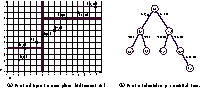
\includegraphics[scale=4.8]{img/kdt/dom-kd}
  \caption{Exemplo de pontos indexados por uma \kdtree{}.}
  \label{fig:kdom-kd}
\end{figure}

A Figura~\ref{fig:query} apresenta um exemplo de operação de verificação de
dominância utilizando uma \dtree{2} como estrutura de indexação.
A área acinzentada não tem intersecção com a área dominada pelo ponto $x$
(área hachurada), portanto as soluções dentro da área acinzentada não são
avaliadas.

\missing{Propor passo-a-passo da operação.}

\begin{figure}[H]
  \centering
  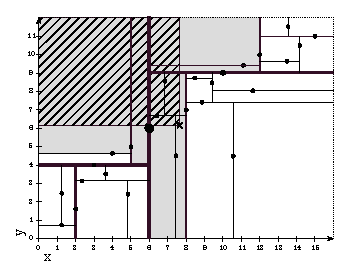
\includegraphics[scale=1.7]{img/kdt/query}
  \caption{Exemplo de operação de verificação de dominância utilizando a \kdtree{}.}
  \label{fig:query}
\end{figure}

Com relação à eficiência da \kdtree{} é importante considerar que não é
recomendável escalar de forma arbitrária o número $k$ de dimensões
indexadas pela \kdtree{}, esperando assim escalar também sua eficiência.
Mesmo que o dado possua todas estas dimensões.
Como regra geral considera-se que um \kdtree{} é adequada para indexar um
conjunto com $n$ pontos se $n$ não for muito maior que $2^k$\cite{toth2004handbook},
caso contrário, a performance da \kdtree{} se assemelhará a de uma busca
linear exaustiva.

Espera-se que a \kdtree{} auxilie as operações de verificação de dominância
\emph{podando} uma grande quantidade de soluções, demandando um menor número
de comparações entre soluções, melhorando assim a performance dos algoritmos.

% Falar um pouco sobre arvore binária.

% Definir a árvore kdtree


% Experimentos
\chapter{Experimentos computacionais}
Vários experimentos computacionais foram realizados com o objetivo de veirficar
a eficiência da indexação multi-dimensional, especialmente em instâncias com
mais de duas dimensões.

\missingt{
  Explicar que são os mesmos tipo de instâncias, mas não o mesmo conjunto, pois
  não foi disponibilizado pelos autores.\\
  Dizer por que da métrica de comparação (hypervolume).\\
}


\missing{Introduzir comentário sobre as instâncias da Bazgan.}
Quatro tipos de instâncias bi-objetivo são consideradas:
\begin{enumerate}
  \item[A)] Aleatórias: $
    p^j_i \in [1, 1000],
    w_i \in [1,1000]$.
  \item[B)] Não-conflitantes: $
    p^1_i \in [111, 1000],\\
    p^2_i \in [p^1_i - 100, p^1_i + 100],\\
    w_i \in [1,1000]$.
  \item[C)] Conflitantes: $
    p^1_i \in [1, 1000],\\
    p^2_i \in [max\{900-p^1_i;1\}, min\{1100-p^1_i, 1000\}],\\
    w_i \in [1,1000]$.
  \item[D)] Conflitantes com pesos correlacionados: $
    p^1_i \in [1, 1000],\\
    p^2_i \in [max\{900-p^1_i;1\}, min\{1100-p^1_i, 1000\}],\\
    w_i \in [p^1_i+p^2_i-200, p^1_i+p^2_i+200]$.
\end{enumerate}
onde $\in [a,b]$ denota uma distribuição uniforme aleatória no intervalo
$[\,b]$.

\missingt{
  Esclarecer os critérios de generalização dos tipos de instância.
}

Para os experimentos com $3$-objetivo considerou-se
a generalização introduzida por~\cite{bazgan2009}
para os tipos $A$ e $C$ e também duas propostas de generalização
para os tipo $B$ e $D$:
\begin{enumerate}
  \item[A)] Aleatórias: $
    p^j_i \in [1, 1000]\\
    w_i \in [1,1000]$
  \item[B)] Não-conflitantes: $
    p^1_i \in [111, 1000],\\
    p^2_i \in [p^1_i - 100, p^1_i + 100],\\
    p^3_i \in [p^1_i - 100, p^1_i + 100],\\
    w_i \in [1,1000]$.
  \item[C)] Conflitantes: $
    p^1_i \in [1, 1000], \;
    p^2_i \in [1, 1001 - p^1_i] \\
    p^3_i \in [max\{900-p^1_i-p^2_i;1\}, min\{1100-p^1_i-p^2_i, 1001-p^1_i\}]\\
    w_i \in [1,1000]$.
  \item[D)] Conflitantes com pesos correlacionados: $
    p^1_i \in [1, 1000]\\
    p^2_i \in [1, 1001 - p^1_i] \\
    p^3_i \in [max\{900-p^1_i-p^2_i;1\}, min\{1100-p^1_i-p^2_i, 1001-p^1_i\}]\\
    w_i \in [p^1_i+p^2_i+p^3_i-200, p^1_i+p^2_i+p^3_i+200]$.
\end{enumerate}
Instâncias do tipo $B$ são consideradas mais fáceis enquanto instâncias do
tipo $D$ são consideradas as mais difíceis.
Para todas as instâncias, atribui-se $W=\frac{1}{2}\floor{\sum^n_{k=1} w^k}$.
Para cada tipo e valor de $n$ dez instâncias foram geradas.


\missingt{Descrever mais as tabelas e resultados.}

\missingt{
Dizer que a seleção dos parametros para o SCE sãos os recomendados pelo autor.\\
Dizer também que varição dos parametros não produzir melhorias consistentes.
}

% Conclusão
\chapter{Conclusão}
O presente trabalho propõe a indexação multidimensional das soluções
do problema da mochila multiobjetivo,
como proposta de aceleração das operações de verificação de dominância de solução.
A operação de verificação de dominância é uma das principais
operações necessárias para a resolução do problema.
A indexação multidimensional das soluções tem por objetivo
reduzir o número de avaliações de soluções necessárias para a execução da operação,
diminuindo consequentemente o tempo computacional
demandado pelo algoritmo.

Há na literatura a proposta de utilização da quadtree como estrutura de dados
de indexação de soluções de problemas multiobjetivo.
Porém a estratégia mostrou-se eficaz apenas em casos bi-objetivos de conjuntos Paretos consideravelmente extensos.
Conjectura-se que essa ineficiência é decorrente
do alto \emph{overhead} da estrutura, especialmente em casos com mais de dois objetivos.

Para que a proposta de indexação fosse possível,
foi definido no presente trabalho um mapeamento entre a operação
de verificação de dominância e o problema da busca de faixa.
O problema de busca de faixa consiste em verificar a existência de pontos em uma determinada
região do espaço multidimensional.
Esse problema é bem conhecido em áreas como computação gráfica, geometria computacional e jogos,
onde a \kdtree{} é geralmente utilizada como estrutura de dados auxiliar.
Sendo assim, a proposta do presente trabalho foi a utilização da \kdtree{}
como estrutura auxiliar da operação de verificação de dominância.

A aplicação e o comportamento da \kdtree{} junto à operação
foram discutidos, bem como os da lista encadeada e da árvore AVL,
estruturas até então utilizadas pela literatura para este fim.
O desempenho da proposta de indexação foi testado no contexto exato e heurístico.

No contexto exato, a proposta foi aplicada ao algoritmo Bazgan,
considerado pela literatura como o mais eficiente atualmente para o problema da mochila multiobjetivo.
A performance do algoritmo foi comparada através de experimentos computacionais.
Para tanto, foi considerada a mesma proposta de instâncias empregada pela literatura,
sendo quatro tipos de instâncias bi-objetivo e dois tipos de instâncias 3-objetivo.
Para o caso 3-objetivo foram ainda propostas mais dois tipos de instâncias,
sendo estas generalizações de seus respectivos casos bi-objetivos.

Os resultados dos experimentos computacionais utilizando o algoritmo Bazgan,
mostraram que a proposta de indexação multidimensional possibilitou o speedup
de até $2.3$ para os casos bi-objetivo, e até $15.5$ para casos 3-objetivo.
A proposta não se mostrou eficiente apenas em instâncias consideradas fáceis,
cujos conjuntos Pareto têm tamanhos consideravelmente reduzidos em relação
às demais instâncias.
Nesses casos, onde se dá a manipulação de poucas soluções,
o \emph{overhead} computacional da \kdtree{} torna sua utilização ineficaz.

No contexto heurístico, a indexação multidimensional
foi aplicada ao algoritmo SCE para o MOKP, proposto também neste trabalho.
Primeiramente o SCE foi adaptado para resolver problemas multiobjetivo.
Para isso, a aptidão das soluções foi definida com base na ordenação
em frontes não dominados.
A aproximação do \paretoset{} foi gerada com o auxílio de um arquivo externo.
Em seguida, foi estabelecida a implementação específica para o MOKP,
definindo-se a operação de geração de solução viável
aleatória e a operação de cruzamento de soluções.

A validade da implementação do algoritmo SCE para o MOKP foi primeiramente
avaliada e comparada com os principais algoritmos da literatura,
não tendo melhores resultados que as
heurísticas de estado-da-arte, porém tendo resultados superiores aos
das heurísticas mais antigas.

Os experimentos computacionais no contexto heurístico
foram realizados sobre o conjunto de 6 instâncias,
utilizado pela literatura para avaliar a performance de heurísticas para o MOKP.
Apesar de reduzir consideravelmente o número de avaliações de soluções,
a utilização da \kdtree{} não apresentou eficiência relevante quanto ao tempo computacional
na abordagem heurística, tendo pior performance nas instâncias com \paretoset{}
relativamente pequenos.

Pode-se concluir que a utilização da \kdtree{} é capaz de reduzir consideravelmente
o número de avaliações de soluções na maioria dos casos, além de também reduzir o tempo computacional
demandado em casos em que é necessário executar a verificação de dominância em grandes
conjuntos de solução.
Os resultados evidenciam ser indispensável
a utilização de uma estrutura de indexação multidimensional,
nos casos de problemas com mais de 2 objetivos com grandes
conjuntos de solução.
Vale ressaltar que os algoritmos não foram alterados, somente
a forma de indexação das soluções.

%\missingf{afirmacao forte: "Segundo os resultados, a utilização de uma estrutura de indexação multidimensional
%mostra-se indispensável no caso de problemas com mais de 2 objetivos com grandes
%conjuntos de solução." em vez de mostra, alterei para evidencia... 
%
%\resp Ok. Melhor.}

Notou-se porém, que em casos onde o número de soluções manipuladas é pequeno, a utilização
da \kdtree{} não é recomendável, pois apesar de apresentar redução no número de
avaliações, o \emph{overhead} da estrutura dificulta uma redução no tempo computacional demandado.

Como trabalhos futuros pretende-se verificar a performance da \kdtree{} em outros problemas
multiobjetivos, bem como comparar com outras estruturas, inclusive com a ND-Tree, proposta
em~\cite{jaszkiewicz2017} como estrutura de dados para auxiliar a operação de verificação de dominância.
Pretende-se também investigar a aplicabilidade de outras estruturas de indexação
multidimensional ou mesmo a proposta de uma específica para conjuntos Pareto de problemas multiobjetivos.

Pretende-se também aprimorar a implementação do SCE para o MOKP.
Uma possibilidade seria o aperfeiçoamento das soluções
através da utilização de conhecimentos específicos do problema.
Outra possibilidade seria realizando um pré-processamento sobre o problema inicial,
transformando-o em um problema mais simples ou dividindo-o em sub-problemas
menores.


\missingf{Sugiro expandir a discussão de trabalhos futuros}

\missingf{ na verdade acho que a Conclusao tem que ser expandida como um todo. Tá parecendo conclusao de artigo, que tem limitacao de espaço. Vc poderia falar mais de cada um dos itens comentados, até apresentar exemplos para esclarecer os leitores.}


\postextual

\bibliography{tex/references}

\end{document}
